%%
%% This is file `sample-sigconf-authordraft.tex',
%% generated with the docstrip utility.
%%
%% The original source files were:
%%
%% samples.dtx  (with options: `all,proceedings,bibtex,authordraft')
%% 
%% IMPORTANT NOTICE:
%% 
%% For the copyright see the source file.
%% 
%% Any modified versions of this file must be renamed
%% with new filenames distinct from sample-sigconf-authordraft.tex.
%% 
%% For distribution of the original source see the terms
%% for copying and modification in the file samples.dtx.
%% 
%% This generated file may be distributed as long as the
%% original source files, as listed above, are part of the
%% same distribution. (The sources need not necessarily be
%% in the same archive or directory.)
%%
%%
%% Commands for TeXCount
%TC:macro \cite [option:text,text]
%TC:macro \citep [option:text,text]
%TC:macro \citet [option:text,text]
%TC:envir table 0 1
%TC:envir table* 0 1
%TC:envir tabular [ignore] word
%TC:envir displaymath 0 word
%TC:envir math 0 word
%TC:envir comment 0 0
%%
%% The first command in your LaTeX source must be the \documentclass
%% command.
%%
%% For submission and review of your manuscript please change the
%% command to \documentclass[manuscript, screen, review]{acmart}.
%%
%% When submitting camera ready or to TAPS, please change the command
%% to \documentclass[sigconf]{acmart} or whichever template is required
%% for your publication.
%%
%%
%\documentclass[sigconf,authordraft]{acmart}
\documentclass[sigconf,review,anonymous]{acmart}
%%
%% \BibTeX command to typeset BibTeX logo in the docs
\AtBeginDocument{%
  \providecommand\BibTeX{{%
    Bib\TeX}}}

%% Rights management information.  This information is sent to you
%% when you complete the rights form.  These commands have SAMPLE
%% values in them; it is your responsibility as an author to replace
%% the commands and values with those provided to you when you
%% complete the rights form.
\setcopyright{acmlicensed}
\copyrightyear{2018}
\acmYear{2018}
\acmDOI{XXXXXXX.XXXXXXX}
%% These commands are for a PROCEEDINGS abstract or paper.
\acmConference[Conference acronym 'XX]{Make sure to enter the correct
  conference title from your rights confirmation email}{June 03--05,
  2018}{Woodstock, NY}
%%
%%  Uncomment \acmBooktitle if the title of the proceedings is different
%%  from ``Proceedings of ...''!
%%
%%\acmBooktitle{Woodstock '18: ACM Symposium on Neural Gaze Detection,
%%  June 03--05, 2018, Woodstock, NY}
\acmISBN{978-1-4503-XXXX-X/2018/06}


%%
%% Submission ID.
%% Use this when submitting an article to a sponsored event. You'll
%% receive a unique submission ID from the organizers
%% of the event, and this ID should be used as the parameter to this command.
%%\acmSubmissionID{123-A56-BU3}

%%
%% For managing citations, it is recommended to use bibliography
%% files in BibTeX format.
%%
%% You can then either use BibTeX with the ACM-Reference-Format style,
%% or BibLaTeX with the acmnumeric or acmauthoryear sytles, that include
%% support for advanced citation of software artefact from the
%% biblatex-software package, also separately available on CTAN.
%%
%% Look at the sample-*-biblatex.tex files for templates showcasing
%% the biblatex styles.
%%

%%
%% The majority of ACM publications use numbered citations and
%% references.  The command \citestyle{authoryear} switches to the
%% "author year" style.
%%
%% If you are preparing content for an event
%% sponsored by ACM SIGGRAPH, you must use the "author year" style of
%% citations and references.
%% Uncommenting
%% the next command will enable that style.
%%\citestyle{acmauthoryear}


%%
%% end of the preamble, start of the body of the document source.
\begin{document}

%%
%% The "title" command has an optional parameter,
%% allowing the author to define a "short title" to be used in page headers.
\title{Personalizing POI Descriptions with LLMs: A Study of User Perceptions and Informational Value}

%%
%% The "author" command and its associated commands are used to define
%% the authors and their affiliations.
%% Of note is the shared affiliation of the first two authors, and the
%% "authornote" and "authornotemark" commands
%% used to denote shared contribution to the research.
\author{Ben Trovato}
\authornote{Both authors contributed equally to this research.}
\email{trovato@corporation.com}
\orcid{1234-5678-9012}
\author{G.K.M. Tobin}
\authornotemark[1]
\email{webmaster@marysville-ohio.com}
\affiliation{%
  \institution{Institute for Clarity in Documentation}
  \city{Dublin}
  \state{Ohio}
  \country{USA}
}

\author{Lars Th{\o}rv{\"a}ld}
\affiliation{%
  \institution{The Th{\o}rv{\"a}ld Group}
  \city{Hekla}
  \country{Iceland}}
\email{larst@affiliation.org}

\author{Valerie B\'eranger}
\affiliation{%
  \institution{Inria Paris-Rocquencourt}
  \city{Rocquencourt}
  \country{France}
}

\author{Aparna Patel}
\affiliation{%
 \institution{Rajiv Gandhi University}
 \city{Doimukh}
 \state{Arunachal Pradesh}
 \country{India}}

\author{Huifen Chan}
\affiliation{%
  \institution{Tsinghua University}
  \city{Haidian Qu}
  \state{Beijing Shi}
  \country{China}}

\author{Charles Palmer}
\affiliation{%
  \institution{Palmer Research Laboratories}
  \city{San Antonio}
  \state{Texas}
  \country{USA}}
\email{cpalmer@prl.com}

\author{John Smith}
\affiliation{%
  \institution{The Th{\o}rv{\"a}ld Group}
  \city{Hekla}
  \country{Iceland}}
\email{jsmith@affiliation.org}

\author{Julius P. Kumquat}
\affiliation{%
  \institution{The Kumquat Consortium}
  \city{New York}
  \country{USA}}
\email{jpkumquat@consortium.net}

%%
%% By default, the full list of authors will be used in the page
%% headers. Often, this list is too long, and will overlap
%% other information printed in the page headers. This command allows
%% the author to define a more concise list
%% of authors' names for this purpose.
\renewcommand{\shortauthors}{Trovato et al.}

%%
%% The abstract is a short summary of the work to be presented in the
%% article.
\begin{abstract}
 Personalization is essential for enhancing user engagement with travel-related content. This study investigates the effectiveness of AI-generated descriptions for Points of Interest (POIs), including hotels, restaurants, museums, and gardens, by adapting content to better align with individual user preferences. A prototype system was developed, allowing users to input their preferences and interests, after which they were presented with both original and LLM-adapted POI descriptions. Participants were then asked to rate the descriptions based on their alignment with personal interests and familiarity with the locations. The study aims to evaluate the impact of personalized descriptions on user acceptance and perceived relevance, offering insights into the potential of large language models for enhancing tourism and travel experiences. The findings reveal key factors influencing user preferences and provide recommendations for improving AI-driven content personalization strategies.
\end{abstract}

%%
%% The code below is generated by the tool at http://dl.acm.org/ccs.cfm.
%% Please copy and paste the code instead of the example below.
%%
\begin{CCSXML}
<ccs2012>
   <concept>
	<concept_id>10003120.10003121.10003122.10003334</concept_id>
	<concept_desc>Human-centered computing~User studies</concept_desc>
	<concept_significance>300</concept_significance>
	</concept>
	<concept>
	<concept_id>10003120.10003123.10010860.10010859</concept_id>
	<concept_desc>Human-centered computing~User centered design</concept_desc>
	<concept_significance>500</concept_significance>
	</concept>
 </ccs2012>
\end{CCSXML}

\ccsdesc[500]{Human-centered computing~User centered design}
\ccsdesc[300]{Human-centered computing~User studies}

%%
%% Keywords. The author(s) should pick words that accurately describe
%% the work being presented. Separate the keywords with commas.
\keywords{poi adaptation, LLM-generated content, ai-driven descriptions, content personalization}
%% A "teaser" image appears between the author and affiliation
%% information and the body of the document, and typically spans the
%% page.
%\begin{teaserfigure}
 % 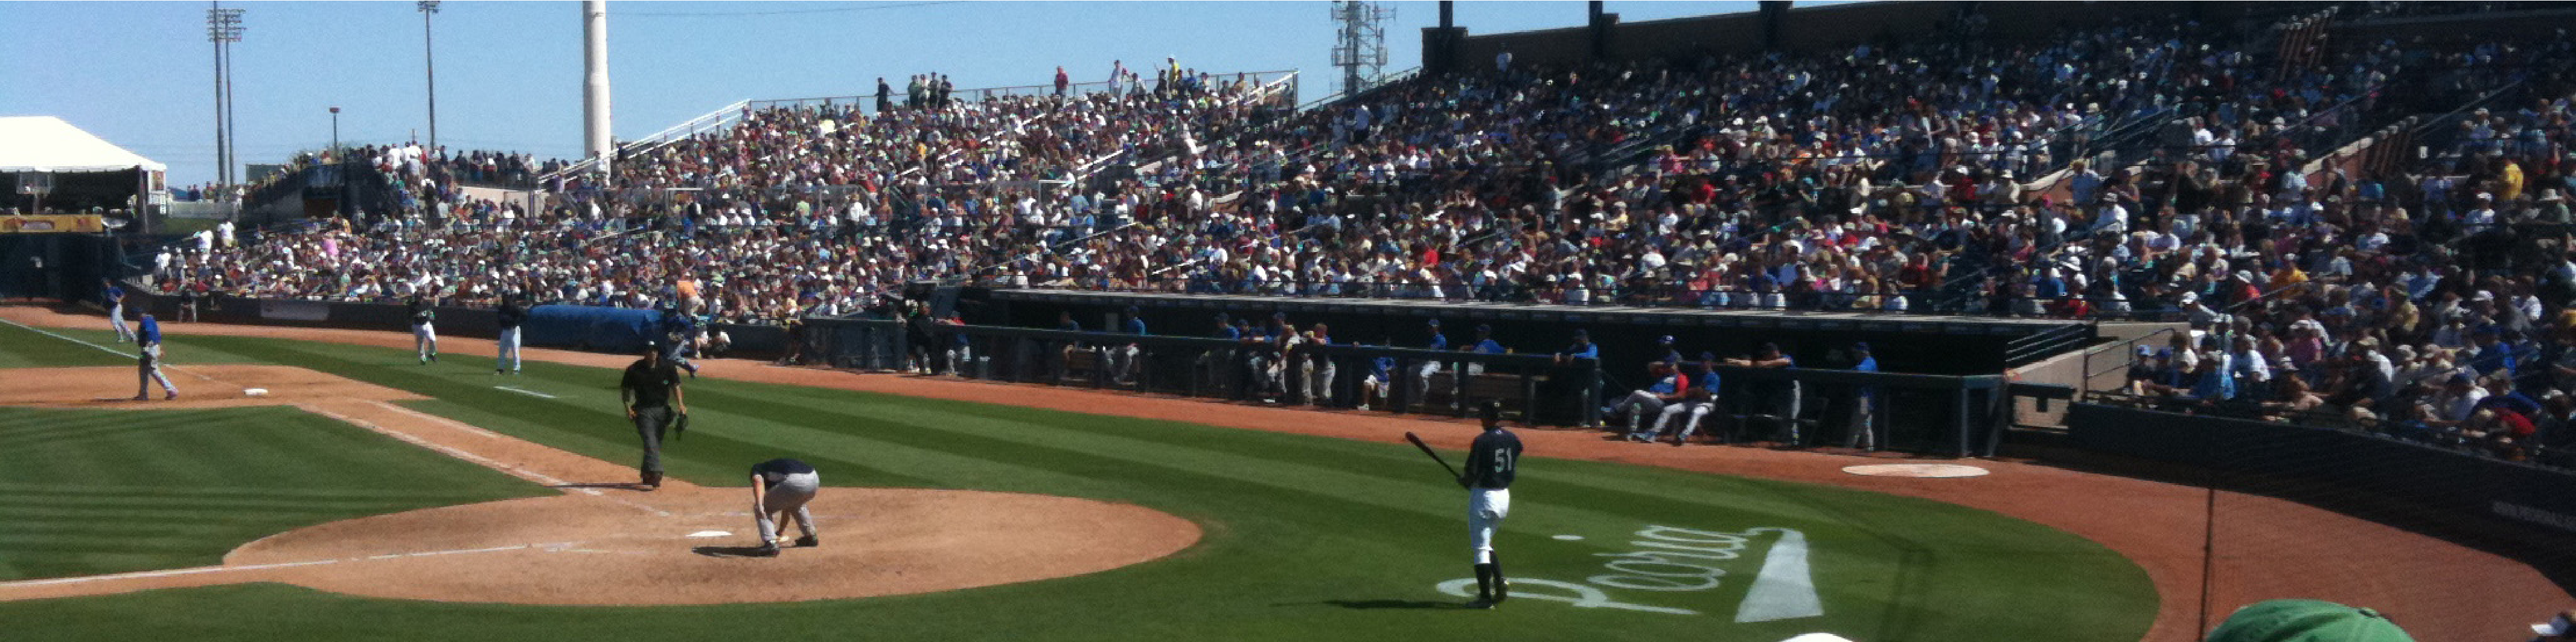
\includegraphics[width=\textwidth]{sampleteaser}
  %\caption{Seattle Mariners at Spring Training, 2010.}
  %\Description{Enjoying the baseball game from the third-base
  %seats. Ichiro Suzuki preparing to bat.}
  %\label{fig:teaser}
%\end{teaserfigure}

\received{20 February 2007}
\received[revised]{12 March 2009}
\received[accepted]{5 June 2009}

%%
%% This command processes the author and affiliation and title
%% information and builds the first part of the formatted document.
\maketitle

\section{Introduction}
Personalization has become a key factor in improving user engagement in various digital experiences, including travel and tourism. As travellers seek more relevant and tailored recommendations, AI advancements, particularly large language models (LLM), presents new opportunities to adapt content to align with individual preferences dynamically. One such application is personalized descriptions of Points of Interest (POIs), such as hotels, restaurants, museums, and gardens. Although traditional POI descriptions are often static and generalized, AI-driven personalization can refine these descriptions to match user-specific interests, past experiences, and contextual relevance, enhancing both engagement and comprehension.

Much prior research has focused on POI recommendation and ranking systems, where AI models suggest locations based on user preferences, behaviors, and contextual factors. However, less attention has been given to how the content of each POI itself can be adapted to better engage users. When individuals access POI descriptions, the same information is typically presented to all users, despite variations in their backgrounds, interests, and motivations to visit a place. For example, a museum description could emphasize historical significance for a history enthusiast while focusing on interactive exhibits for a family traveler. Generative AI and LLMs provide a unique opportunity to dynamically tailor content without altering its factual meaning, ensuring that the description remains relevant and appealing to different audiences.

To explore this potential, we developed a prototype system that allows users to enter their preferences and interests and then dynamically presents them with two versions of each POI description: the original and an LLM-adapted version. Participants were asked to evaluate the descriptions based on alignment with their preferences, perceived appeal, and familiarity with the location. The key objective is to assess whether AI-generated adaptations are acceptable and meaningful, effectively convey the original value of POI, and improve user engagement.

This study contributes to the growing field of AI-powered content personalization in tourism by investigating the role of LLMs in dynamic adaptation of textual content. By analyzing participant feedback, we aim to provide insight into how AI-generated descriptions can improve engagement while preserving accuracy and authenticity.

The remainder of this paper is structured as follows. Section 2 discusses related work in AI-driven personalization, POI recommendation and ranking systems, and content adaptation techniques. Section 3 details our methodology, including the experimental setup, data collection process, and evaluation metrics. Section 4 presents the results and the analysis of the user preferences and satisfaction. Finally, Section 5 discusses the implications of our findings, potential improvements, and future research directions.

\section{Related work}


\section{Methodology}
To assess the effectiveness of LLM-generated adaptations of POI descriptions, we conducted a user study where participants evaluated both original and AI-adapted descriptions based on their alignment with personal preferences, perceived appeal, and ability to convey the original value of the POI. This section details the study design, participant recruitment, evaluation criteria.

\subsection{Study Design}
The study was structured as a within-subjects experiment, where each participant evaluated multiple POIs and compared both original and AI-adapted descriptions. This approach allowed for direct comparisons between static and personalized content while minimizing individual biases. The study included ten POIs, categorized into five different types—hotels, restaurants, museums, gardens, and landmarks—ensuring a diverse representation of travel-related locations. Each category contained two POIs, carefully selected to provide a balanced mix of well-known and lesser-known places.

For each POI, participants were shown two descriptions side by side, but they were not informed which one was AI-adapted and which one was the original. One description was the original, unmodified version, while the other was dynamically generated using an LLM, tailored to the participant’s previously provided interests and preferences. To reduce order effects, the position of the AI-adapted and original descriptions was randomized for each POI. The study was designed to assess whether AI-generated adaptations were both meaningful and engaging while preserving the original value of the POI. It also examined whether personalized descriptions increased user interest in visiting the locations.

\subsection{Procedure}
The study began with a consent form, where participants were informed about the purpose of the study, the voluntary nature of participation, and data confidentiality. After providing consent, participants proceeded to a background and preference survey. This survey collected demographic information such as age, gender, nationality, profession, and current city. Additionally, participants specified their travel-related preferences, selecting from a list of hobbies, preferred travel styles, and key tourism interests. This input was later used to personalize POI descriptions for the evaluation phase.

Once the survey was completed, participants moved on to the main evaluation task, where they were presented with ten POIs, each accompanied by an image. For each POI, they reviewed two descriptions (one original, one AI-adapted) without knowing which was which. Participants were then asked to evaluate each description individually based on clarity, trustworthiness, and effectiveness in conveying the significance of the POI.

Following the individual assessment, participants completed a comparative evaluation, where they indicated which description was more engaging, informative, appealing, and likely to encourage them to visit the location. To further understand how prior knowledge influenced perception, participants were also asked to report their familiarity with each POI, specifying whether they had previously visited it, heard about it, or were entirely unfamiliar with it.

Upon completing evaluations for all ten POIs, participants submitted their responses, concluding the study. The entire process took approximately 20 to 30 minutes, with minor variations depending on reading speed and response time. All data was collected anonymously, ensuring participant privacy and compliance with ethical research standards.
\begin{figure*}[h]
  \centering
  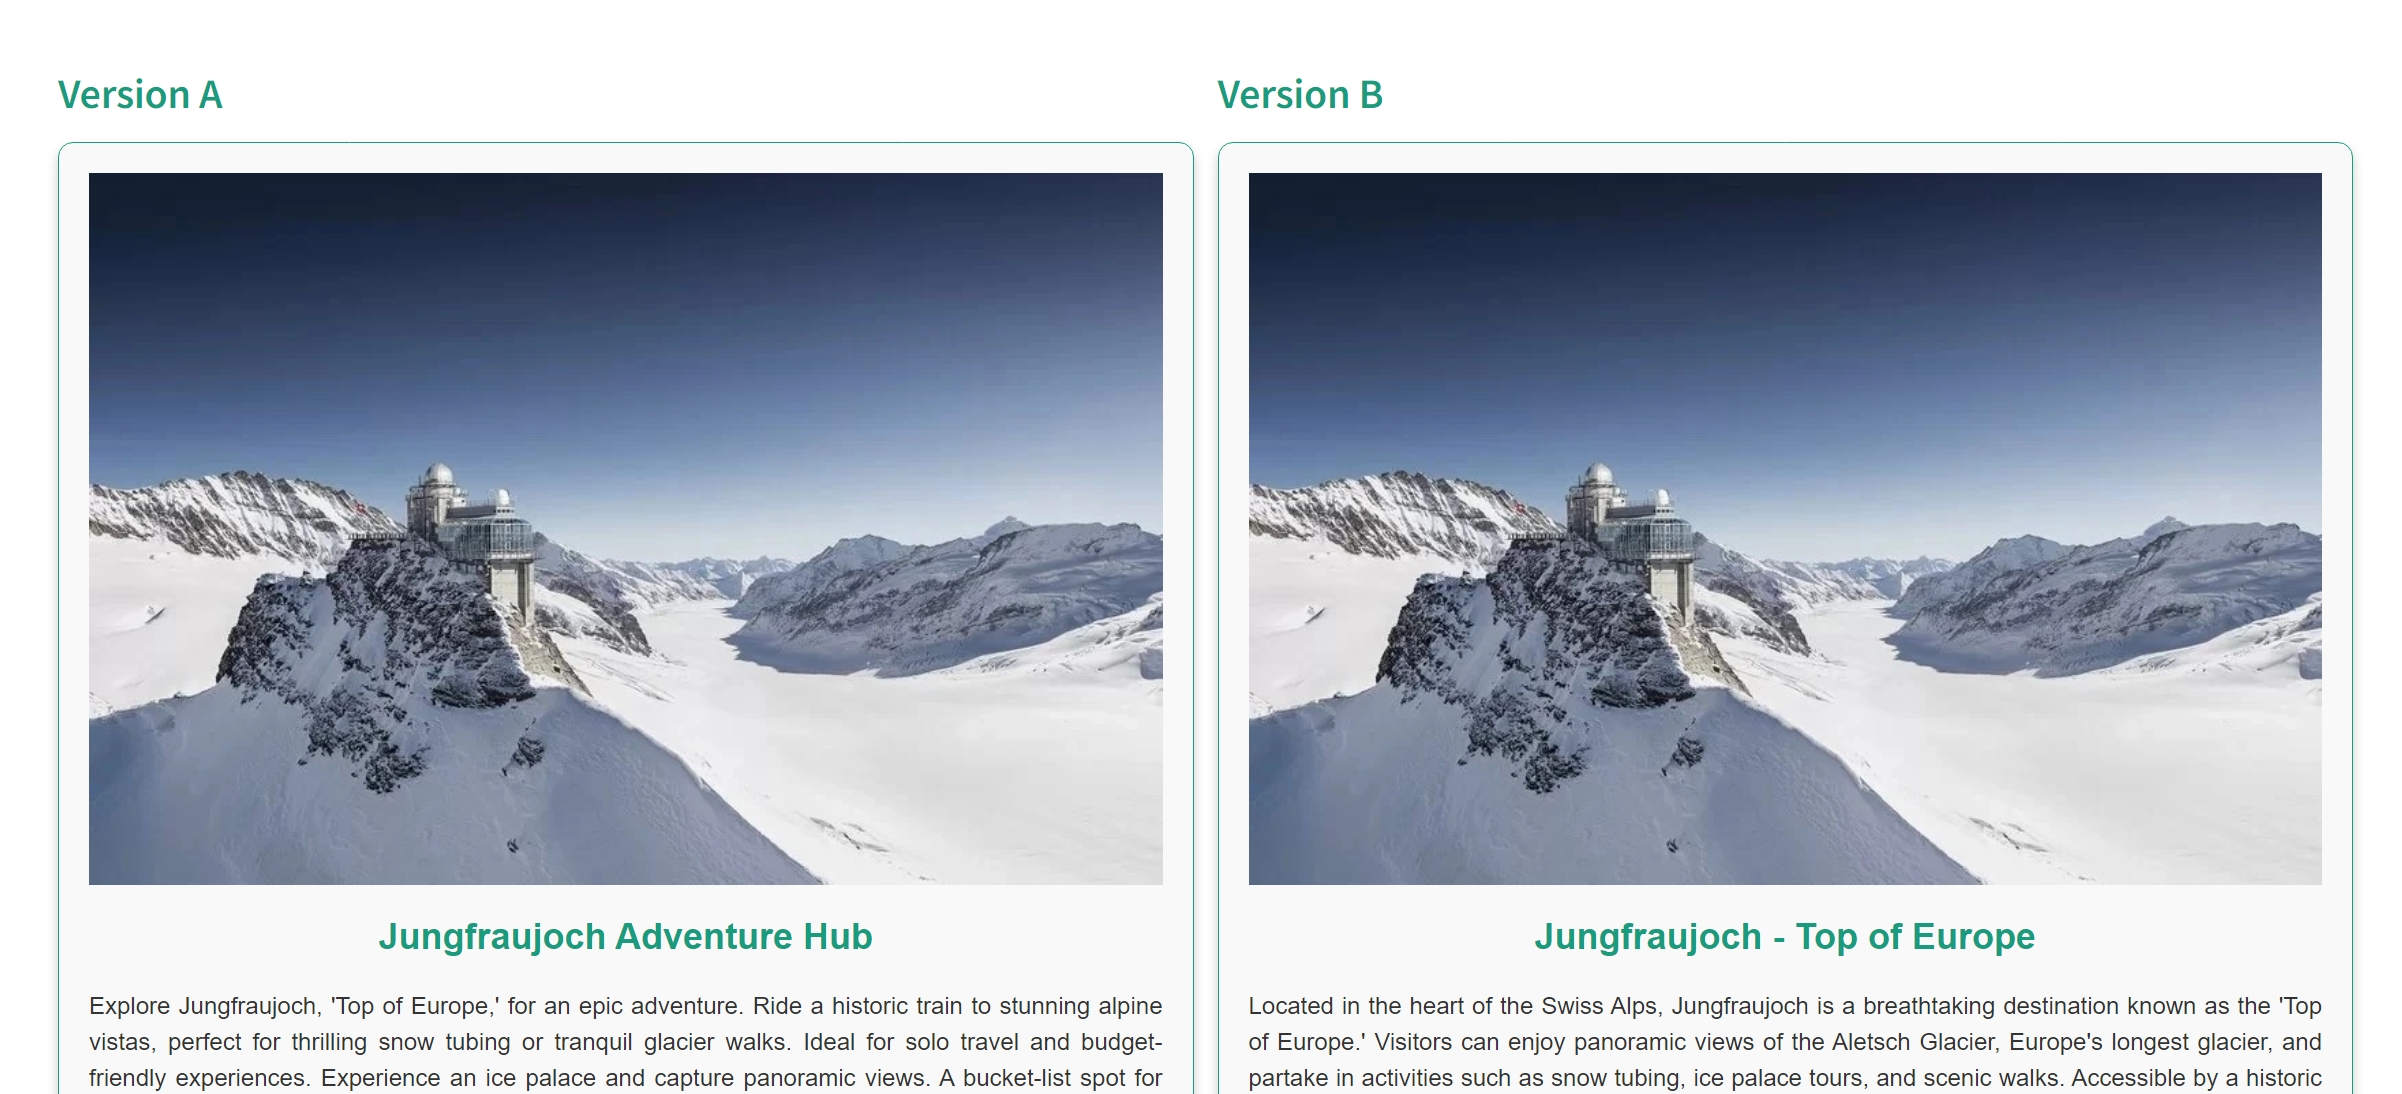
\includegraphics[width=\linewidth]{figures/eval1.jpeg}
  \caption{Two versions of POIs as shown to users}
  \Description{two versions of POIs as shown to users}
\end{figure*}
\subsection{Participants}

The study recruited X participants through email and direct messages to friends, family, and colleagues. The participant pool was designed to include a diverse range of individuals with varying backgrounds and travel preferences to ensure the findings would be broadly applicable. The age of participants ranged from X to X years (M = 37.18, SD = 4.77). Participants were required to be at least 18 years old and have a basic level of English proficiency to ensure they could effectively engage with the POI descriptions. No specific travel experience was required, as the study aimed to assess how AI-generated descriptions appeal to both frequent and occasional travelers.

In addition to specifying the {\itshape template style} to be used in
formatting your work, there are a number of {\itshape template parameters}
which modify some part of the applied template style. A complete list
of these parameters can be found in the {\itshape \LaTeX\ User's Guide.}

Frequently-used parameters, or combinations of parameters, include:
\begin{itemize}
\item {\texttt{anonymous,review}}: Suitable for a ``double-anonymous''
  conference submission. Anonymizes the work and includes line
  numbers. Use with the \texttt{\string\acmSubmissionID} command to print the
  submission's unique ID on each page of the work.
\item{\texttt{authorversion}}: Produces a version of the work suitable
  for posting by the author.
\item{\texttt{screen}}: Produces colored hyperlinks.
\end{itemize}

This document uses the following string as the first command in the
source file:
\begin{verbatim}
\documentclass[sigconf,authordraft]{acmart}
\end{verbatim}





\section{Acknowledgments}

Identification of funding sources and other support, and thanks to
individuals and groups that assisted in the research and the
preparation of the work should be included in an acknowledgment
section, which is placed just before the reference section in your
document.

This section has a special environment:
\begin{verbatim}
  \begin{acks}
  ...
  \end{acks}
\end{verbatim}
so that the information contained therein can be more easily collected
during the article metadata extraction phase, and to ensure
consistency in the spelling of the section heading.

Authors should not prepare this section as a numbered or unnumbered {\verb|\section|}; please use the ``{\verb|acks|}'' environment.

\section{Appendices}

If your work needs an appendix, add it before the
``\verb|\end{document}|'' command at the conclusion of your source
document.

Start the appendix with the ``\verb|appendix|'' command:
\begin{verbatim}
  \appendix
\end{verbatim}
and note that in the appendix, sections are lettered, not
numbered. This document has two appendices, demonstrating the section
and subsection identification method.

\section{Multi-language papers}

Papers may be written in languages other than English or include
titles, subtitles, keywords and abstracts in different languages (as a
rule, a paper in a language other than English should include an
English title and an English abstract).  Use \verb|language=...| for
every language used in the paper.  The last language indicated is the
main language of the paper.  For example, a French paper with
additional titles and abstracts in English and German may start with
the following command
\begin{verbatim}
\documentclass[sigconf, language=english, language=german,
               language=french]{acmart}
\end{verbatim}

The title, subtitle, keywords and abstract will be typeset in the main
language of the paper.  The commands \verb|\translatedXXX|, \verb|XXX|
begin title, subtitle and keywords, can be used to set these elements
in the other languages.  The environment \verb|translatedabstract| is
used to set the translation of the abstract.  These commands and
environment have a mandatory first argument: the language of the
second argument.  See \verb|sample-sigconf-i13n.tex| file for examples
of their usage.

\section{SIGCHI Extended Abstracts}

The ``\verb|sigchi-a|'' template style (available only in \LaTeX\ and
not in Word) produces a landscape-orientation formatted article, with
a wide left margin. Three environments are available for use with the
``\verb|sigchi-a|'' template style, and produce formatted output in
the margin:
\begin{description}
\item[\texttt{sidebar}:]  Place formatted text in the margin.
\item[\texttt{marginfigure}:] Place a figure in the margin.
\item[\texttt{margintable}:] Place a table in the margin.
\end{description}

%%
%% The acknowledgments section is defined using the "acks" environment
%% (and NOT an unnumbered section). This ensures the proper
%% identification of the section in the article metadata, and the
%% consistent spelling of the heading.
\begin{acks}
To Robert, for the bagels and explaining CMYK and color spaces.
\end{acks}

%%
%% The next two lines define the bibliography style to be used, and
%% the bibliography file.
\bibliographystyle{ACM-Reference-Format}
\bibliography{sample-base}


%%
%% If your work has an appendix, this is the place to put it.
\appendix

\section{Research Methods}

\subsection{Part One}

Lorem ipsum dolor sit amet, consectetur adipiscing elit. Morbi
malesuada, quam in pulvinar varius, metus nunc fermentum urna, id
sollicitudin purus odio sit amet enim. Aliquam ullamcorper eu ipsum
vel mollis. Curabitur quis dictum nisl. Phasellus vel semper risus, et
lacinia dolor. Integer ultricies commodo sem nec semper.

\subsection{Part Two}

Etiam commodo feugiat nisl pulvinar pellentesque. Etiam auctor sodales
ligula, non varius nibh pulvinar semper. Suspendisse nec lectus non
ipsum convallis congue hendrerit vitae sapien. Donec at laoreet
eros. Vivamus non purus placerat, scelerisque diam eu, cursus
ante. Etiam aliquam tortor auctor efficitur mattis.

\section{Online Resources}

Nam id fermentum dui. Suspendisse sagittis tortor a nulla mollis, in
pulvinar ex pretium. Sed interdum orci quis metus euismod, et sagittis
enim maximus. Vestibulum gravida massa ut felis suscipit
congue. Quisque mattis elit a risus ultrices commodo venenatis eget
dui. Etiam sagittis eleifend elementum.

Nam interdum magna at lectus dignissim, ac dignissim lorem
rhoncus. Maecenas eu arcu ac neque placerat aliquam. Nunc pulvinar
massa et mattis lacinia.

\end{document}
\endinput
%%
%% End of file `sample-sigconf-authordraft.tex'.
